\documentclass[twoside]{book}

% Packages required by doxygen
\usepackage{fixltx2e}
\usepackage{calc}
\usepackage{doxygen}
\usepackage[export]{adjustbox} % also loads graphicx
\usepackage{graphicx}
\usepackage[utf8]{inputenc}
\usepackage{makeidx}
\usepackage{multicol}
\usepackage{multirow}
\PassOptionsToPackage{warn}{textcomp}
\usepackage{textcomp}
\usepackage[nointegrals]{wasysym}
\usepackage[table]{xcolor}

% Font selection
\usepackage[T1]{fontenc}
\usepackage[scaled=.90]{helvet}
\usepackage{courier}
\usepackage{amssymb}
\usepackage{sectsty}
\renewcommand{\familydefault}{\sfdefault}
\allsectionsfont{%
  \fontseries{bc}\selectfont%
  \color{darkgray}%
}
\renewcommand{\DoxyLabelFont}{%
  \fontseries{bc}\selectfont%
  \color{darkgray}%
}
\newcommand{\+}{\discretionary{\mbox{\scriptsize$\hookleftarrow$}}{}{}}

% Page & text layout
\usepackage{geometry}
\geometry{%
  a4paper,%
  top=2.5cm,%
  bottom=2.5cm,%
  left=2.5cm,%
  right=2.5cm%
}
\tolerance=750
\hfuzz=15pt
\hbadness=750
\setlength{\emergencystretch}{15pt}
\setlength{\parindent}{0cm}
\setlength{\parskip}{3ex plus 2ex minus 2ex}
\makeatletter
\renewcommand{\paragraph}{%
  \@startsection{paragraph}{4}{0ex}{-1.0ex}{1.0ex}{%
    \normalfont\normalsize\bfseries\SS@parafont%
  }%
}
\renewcommand{\subparagraph}{%
  \@startsection{subparagraph}{5}{0ex}{-1.0ex}{1.0ex}{%
    \normalfont\normalsize\bfseries\SS@subparafont%
  }%
}
\makeatother

% Headers & footers
\usepackage{fancyhdr}
\pagestyle{fancyplain}
\fancyhead[LE]{\fancyplain{}{\bfseries\thepage}}
\fancyhead[CE]{\fancyplain{}{}}
\fancyhead[RE]{\fancyplain{}{\bfseries\leftmark}}
\fancyhead[LO]{\fancyplain{}{\bfseries\rightmark}}
\fancyhead[CO]{\fancyplain{}{}}
\fancyhead[RO]{\fancyplain{}{\bfseries\thepage}}
\fancyfoot[LE]{\fancyplain{}{}}
\fancyfoot[CE]{\fancyplain{}{}}
\fancyfoot[RE]{\fancyplain{}{\bfseries\scriptsize Generated by Doxygen }}
\fancyfoot[LO]{\fancyplain{}{\bfseries\scriptsize Generated by Doxygen }}
\fancyfoot[CO]{\fancyplain{}{}}
\fancyfoot[RO]{\fancyplain{}{}}
\renewcommand{\footrulewidth}{0.4pt}
\renewcommand{\chaptermark}[1]{%
  \markboth{#1}{}%
}
\renewcommand{\sectionmark}[1]{%
  \markright{\thesection\ #1}%
}

% Indices & bibliography
\usepackage{natbib}
\usepackage[titles]{tocloft}
\setcounter{tocdepth}{3}
\setcounter{secnumdepth}{5}
\makeindex

% Custom commands
\newcommand{\clearemptydoublepage}{%
  \newpage{\pagestyle{empty}\cleardoublepage}%
}

\usepackage{caption}
\captionsetup{labelsep=space,justification=centering,font={bf},singlelinecheck=off,skip=4pt,position=top}

%===== C O N T E N T S =====

\begin{document}

% Titlepage & ToC
\pagenumbering{roman}
\begin{titlepage}
\vspace*{7cm}
\begin{center}%
{\Large V\+D\+S\+Project }\\
\vspace*{1cm}
{\large Generated by Doxygen 1.8.11}\\
\end{center}
\end{titlepage}
\clearemptydoublepage
\tableofcontents
\clearemptydoublepage
\pagenumbering{arabic}

%--- Begin generated contents ---
\chapter{Hierarchical Index}
\section{Class Hierarchy}
This inheritance list is sorted roughly, but not completely, alphabetically\+:\begin{DoxyCompactList}
\item \contentsline{section}{ska\+:\+:detailv3\+:\+:Assign\+If\+True$<$ T, bool $>$}{\pageref{structska_1_1detailv3_1_1AssignIfTrue}}{}
\item \contentsline{section}{ska\+:\+:detailv3\+:\+:Assign\+If\+True$<$ T, false $>$}{\pageref{structska_1_1detailv3_1_1AssignIfTrue_3_01T_00_01false_01_4}}{}
\item \contentsline{section}{Class\+Project\+:\+:B\+D\+D\+\_\+\+Node}{\pageref{structClassProject_1_1BDD__Node}}{}
\item \contentsline{section}{Class\+Project\+:\+:B\+D\+D\+Comparer}{\pageref{structClassProject_1_1BDDComparer}}{}
\item \contentsline{section}{Class\+Project\+:\+:Bdd\+Dumper}{\pageref{classClassProject_1_1BddDumper}}{}
\begin{DoxyCompactList}
\item \contentsline{section}{Class\+Project\+:\+:Dot\+Bdd\+Dumper}{\pageref{classClassProject_1_1DotBddDumper}}{}
\item \contentsline{section}{Class\+Project\+:\+:Text\+Bdd\+Dumper}{\pageref{classClassProject_1_1TextBddDumper}}{}
\end{DoxyCompactList}
\item \contentsline{section}{Class\+Project\+:\+:B\+D\+D\+Hasher}{\pageref{structClassProject_1_1BDDHasher}}{}
\item \contentsline{section}{Class\+Project\+:\+:Bdd\+Node\+Dumper}{\pageref{classClassProject_1_1BddNodeDumper}}{}
\item \contentsline{section}{bench\+\_\+circuit\+\_\+manager}{\pageref{classbench__circuit__manager}}{}
\item \contentsline{section}{bench\+\_\+format\+:\+:bench\+\_\+node\+\_\+type}{\pageref{structbench__format_1_1bench__node__type}}{}
\item \contentsline{section}{circuit\+\_\+node\+\_\+type}{\pageref{structcircuit__node__type}}{}
\item \contentsline{section}{circuit\+\_\+to\+\_\+\+B\+D\+D\+\_\+manager}{\pageref{classcircuit__to__BDD__manager}}{}
\item \contentsline{section}{ska\+:\+:detailv3\+:\+:sherwood\+\_\+v3\+\_\+table$<$ T, Find\+Key, Argument\+Hash, Hasher, Argument\+Equal, Equal, Argument\+Alloc, Entry\+Alloc $>$\+:\+:convertible\+\_\+to\+\_\+iterator}{\pageref{structska_1_1detailv3_1_1sherwood__v3__table_1_1convertible__to__iterator}}{}
\item \contentsline{section}{ska\+:\+:flat\+\_\+hash\+\_\+map$<$ K, V, H, E, A $>$\+:\+:convertible\+\_\+to\+\_\+value}{\pageref{structska_1_1flat__hash__map_1_1convertible__to__value}}{}
\item E\begin{DoxyCompactList}
\item \contentsline{section}{ska\+:\+:detailv3\+:\+:functor\+\_\+storage$<$ bool, E $>$}{\pageref{structska_1_1detailv3_1_1functor__storage}}{}
\begin{DoxyCompactList}
\item \contentsline{section}{ska\+:\+:detailv3\+:\+:Key\+Or\+Value\+Equality$<$ K, std\+:\+:pair$<$ K, V $>$, E $>$}{\pageref{structska_1_1detailv3_1_1KeyOrValueEquality}}{}
\begin{DoxyCompactList}
\item \contentsline{section}{ska\+:\+:detailv3\+:\+:sherwood\+\_\+v3\+\_\+table$<$ std\+:\+:pair$<$ K, V $>$, K, H, detailv3\+:\+:Key\+Or\+Value\+Hasher$<$ K, std\+:\+:pair$<$ K, V $>$, H $>$, E, detailv3\+:\+:Key\+Or\+Value\+Equality$<$ K, std\+:\+:pair$<$ K, V $>$, E $>$, A, std\+:\+:allocator\+\_\+traits$<$ A $>$\+:\+:template rebind\+\_\+alloc$<$ detailv3\+:\+:sherwood\+\_\+v3\+\_\+entry$<$ std\+:\+:pair$<$ K, V $>$ $>$ $>$ $>$}{\pageref{classska_1_1detailv3_1_1sherwood__v3__table}}{}
\begin{DoxyCompactList}
\item \contentsline{section}{ska\+:\+:flat\+\_\+hash\+\_\+map$<$ K, V, H, E, A $>$}{\pageref{classska_1_1flat__hash__map}}{}
\end{DoxyCompactList}
\end{DoxyCompactList}
\item \contentsline{section}{ska\+:\+:detailv3\+:\+:sherwood\+\_\+v3\+\_\+table$<$ T, T, H, detailv3\+:\+:functor\+\_\+storage$<$ size\+\_\+t, H $>$, E, detailv3\+:\+:functor\+\_\+storage$<$ bool, E $>$, A, std\+:\+:allocator\+\_\+traits$<$ A $>$\+:\+:template rebind\+\_\+alloc$<$ detailv3\+:\+:sherwood\+\_\+v3\+\_\+entry$<$ T $>$ $>$ $>$}{\pageref{classska_1_1detailv3_1_1sherwood__v3__table}}{}
\begin{DoxyCompactList}
\item \contentsline{section}{ska\+:\+:flat\+\_\+hash\+\_\+set$<$ T, H, E, A $>$}{\pageref{classska_1_1flat__hash__set}}{}
\end{DoxyCompactList}
\end{DoxyCompactList}
\end{DoxyCompactList}
\item \contentsline{section}{ska\+:\+:detailv3\+:\+:Entry\+Default\+Table$<$ T $>$}{\pageref{structska_1_1detailv3_1_1EntryDefaultTable}}{}
\item \contentsline{section}{ska\+:\+:detailv3\+:\+:functor\+\_\+storage$<$ Result, Result($\ast$)(Args...)$>$}{\pageref{structska_1_1detailv3_1_1functor__storage_3_01Result_00_01Result_07_5_08_07Args_8_8_8_08_4}}{}
\item grammar\begin{DoxyCompactList}
\item \contentsline{section}{skip\+\_\+p\+:\+:skip\+\_\+grammar$<$ Iterator $>$}{\pageref{structskip__p_1_1skip__grammar}}{}
\end{DoxyCompactList}
\item H\begin{DoxyCompactList}
\item \contentsline{section}{ska\+:\+:detailv3\+:\+:functor\+\_\+storage$<$ size\+\_\+t, H $>$}{\pageref{structska_1_1detailv3_1_1functor__storage}}{}
\begin{DoxyCompactList}
\item \contentsline{section}{ska\+:\+:detailv3\+:\+:Key\+Or\+Value\+Hasher$<$ K, std\+:\+:pair$<$ K, V $>$, H $>$}{\pageref{structska_1_1detailv3_1_1KeyOrValueHasher}}{}
\begin{DoxyCompactList}
\item \contentsline{section}{ska\+:\+:detailv3\+:\+:sherwood\+\_\+v3\+\_\+table$<$ std\+:\+:pair$<$ K, V $>$, K, H, detailv3\+:\+:Key\+Or\+Value\+Hasher$<$ K, std\+:\+:pair$<$ K, V $>$, H $>$, E, detailv3\+:\+:Key\+Or\+Value\+Equality$<$ K, std\+:\+:pair$<$ K, V $>$, E $>$, A, std\+:\+:allocator\+\_\+traits$<$ A $>$\+:\+:template rebind\+\_\+alloc$<$ detailv3\+:\+:sherwood\+\_\+v3\+\_\+entry$<$ std\+:\+:pair$<$ K, V $>$ $>$ $>$ $>$}{\pageref{classska_1_1detailv3_1_1sherwood__v3__table}}{}
\end{DoxyCompactList}
\item \contentsline{section}{ska\+:\+:detailv3\+:\+:sherwood\+\_\+v3\+\_\+table$<$ T, T, H, detailv3\+:\+:functor\+\_\+storage$<$ size\+\_\+t, H $>$, E, detailv3\+:\+:functor\+\_\+storage$<$ bool, E $>$, A, std\+:\+:allocator\+\_\+traits$<$ A $>$\+:\+:template rebind\+\_\+alloc$<$ detailv3\+:\+:sherwood\+\_\+v3\+\_\+entry$<$ T $>$ $>$ $>$}{\pageref{classska_1_1detailv3_1_1sherwood__v3__table}}{}
\end{DoxyCompactList}
\end{DoxyCompactList}
\item hash\begin{DoxyCompactList}
\item \contentsline{section}{ska\+:\+:power\+\_\+of\+\_\+two\+\_\+std\+\_\+hash$<$ T $>$}{\pageref{structska_1_1power__of__two__std__hash}}{}
\end{DoxyCompactList}
\item \contentsline{section}{std\+:\+:hash$<$ boost\+:\+:uuids\+:\+:uuid $>$}{\pageref{structstd_1_1hash_3_01boost_1_1uuids_1_1uuid_01_4}}{}
\item \contentsline{section}{ska\+:\+:detailv3\+:\+:Hash\+Policy\+Selector$<$ T, typename $>$}{\pageref{structska_1_1detailv3_1_1HashPolicySelector}}{}
\item \contentsline{section}{ska\+:\+:detailv3\+:\+:Hash\+Policy\+Selector$<$ Argument\+Hash $>$}{\pageref{structska_1_1detailv3_1_1HashPolicySelector}}{}
\item \contentsline{section}{ska\+:\+:detailv3\+:\+:Hash\+Policy\+Selector$<$ H $>$}{\pageref{structska_1_1detailv3_1_1HashPolicySelector}}{}
\item \contentsline{section}{ska\+:\+:detailv3\+:\+:Hash\+Policy\+Selector$<$ T, void\+\_\+t$<$ typename T\+:\+:hash\+\_\+policy $>$ $>$}{\pageref{structska_1_1detailv3_1_1HashPolicySelector_3_01T_00_01void__t_3_01typename_01T_1_1hash__policy_01_4_01_4}}{}
\item \contentsline{section}{Class\+Project\+:\+:Manager\+Interface}{\pageref{classClassProject_1_1ManagerInterface}}{}
\begin{DoxyCompactList}
\item \contentsline{section}{Class\+Project\+:\+:Manager}{\pageref{classClassProject_1_1Manager}}{}
\end{DoxyCompactList}
\item \contentsline{section}{node}{\pageref{structnode}}{}
\item \contentsline{section}{ska\+:\+:power\+\_\+of\+\_\+two\+\_\+hash\+\_\+policy}{\pageref{structska_1_1power__of__two__hash__policy}}{}
\item \contentsline{section}{ska\+:\+:prime\+\_\+number\+\_\+hash\+\_\+policy}{\pageref{structska_1_1prime__number__hash__policy}}{}
\item runtime\+\_\+error\begin{DoxyCompactList}
\item \contentsline{section}{Cicle\+Exception}{\pageref{classCicleException}}{}
\item \contentsline{section}{Dir\+Exception}{\pageref{classDirException}}{}
\item \contentsline{section}{File\+Exception}{\pageref{classFileException}}{}
\item \contentsline{section}{Inexistent\+B\+D\+D\+\_\+\+I\+D\+Exception}{\pageref{classInexistentBDD__IDException}}{}
\item \contentsline{section}{Inexistent\+B\+D\+D\+Label\+Exception}{\pageref{classInexistentBDDLabelException}}{}
\item \contentsline{section}{Inexistent\+Label\+Exception}{\pageref{classInexistentLabelException}}{}
\item \contentsline{section}{Inexistent\+U\+U\+I\+D\+Exception}{\pageref{classInexistentUUIDException}}{}
\item \contentsline{section}{Open\+File\+Exception}{\pageref{classOpenFileException}}{}
\item \contentsline{section}{Syntax\+Exception}{\pageref{classSyntaxException}}{}
\end{DoxyCompactList}
\item \contentsline{section}{ska\+:\+:detailv3\+:\+:sherwood\+\_\+v3\+\_\+entry$<$ T $>$}{\pageref{structska_1_1detailv3_1_1sherwood__v3__entry}}{}
\item \contentsline{section}{ska\+:\+:detailv3\+:\+:sherwood\+\_\+v3\+\_\+entry\+\_\+constexpr$<$ T $>$}{\pageref{structska_1_1detailv3_1_1sherwood__v3__entry__constexpr}}{}
\item template rebind\+\_\+alloc$<$ detailv3\+:\+:sherwood\+\_\+v3\+\_\+entry$<$ std\+:\+:pair$<$ K, V $>$ $>$ $>$\begin{DoxyCompactList}
\item \contentsline{section}{ska\+:\+:detailv3\+:\+:sherwood\+\_\+v3\+\_\+table$<$ std\+:\+:pair$<$ K, V $>$, K, H, detailv3\+:\+:Key\+Or\+Value\+Hasher$<$ K, std\+:\+:pair$<$ K, V $>$, H $>$, E, detailv3\+:\+:Key\+Or\+Value\+Equality$<$ K, std\+:\+:pair$<$ K, V $>$, E $>$, A, std\+:\+:allocator\+\_\+traits$<$ A $>$\+:\+:template rebind\+\_\+alloc$<$ detailv3\+:\+:sherwood\+\_\+v3\+\_\+entry$<$ std\+:\+:pair$<$ K, V $>$ $>$ $>$ $>$}{\pageref{classska_1_1detailv3_1_1sherwood__v3__table}}{}
\end{DoxyCompactList}
\item template rebind\+\_\+alloc$<$ detailv3\+:\+:sherwood\+\_\+v3\+\_\+entry$<$ T $>$ $>$\begin{DoxyCompactList}
\item \contentsline{section}{ska\+:\+:detailv3\+:\+:sherwood\+\_\+v3\+\_\+table$<$ T, T, H, detailv3\+:\+:functor\+\_\+storage$<$ size\+\_\+t, H $>$, E, detailv3\+:\+:functor\+\_\+storage$<$ bool, E $>$, A, std\+:\+:allocator\+\_\+traits$<$ A $>$\+:\+:template rebind\+\_\+alloc$<$ detailv3\+:\+:sherwood\+\_\+v3\+\_\+entry$<$ T $>$ $>$ $>$}{\pageref{classska_1_1detailv3_1_1sherwood__v3__table}}{}
\end{DoxyCompactList}
\item \contentsline{section}{ska\+:\+:detailv3\+:\+:sherwood\+\_\+v3\+\_\+table$<$ T, Find\+Key, Argument\+Hash, Hasher, Argument\+Equal, Equal, Argument\+Alloc, Entry\+Alloc $>$\+:\+:templated\+\_\+iterator$<$ Value\+Type $>$}{\pageref{structska_1_1detailv3_1_1sherwood__v3__table_1_1templated__iterator}}{}
\item \contentsline{section}{ska\+:\+:detailv3\+:\+:sherwood\+\_\+v3\+\_\+table$<$ T, Find\+Key, Argument\+Hash, Hasher, Argument\+Equal, Equal, Argument\+Alloc, Entry\+Alloc $>$\+:\+:templated\+\_\+iterator$<$ value\+\_\+type $>$}{\pageref{structska_1_1detailv3_1_1sherwood__v3__table_1_1templated__iterator}}{}
\item Entry\+Alloc\begin{DoxyCompactList}
\item \contentsline{section}{ska\+:\+:detailv3\+:\+:sherwood\+\_\+v3\+\_\+table$<$ T, Find\+Key, Argument\+Hash, Hasher, Argument\+Equal, Equal, Argument\+Alloc, Entry\+Alloc $>$}{\pageref{classska_1_1detailv3_1_1sherwood__v3__table}}{}
\end{DoxyCompactList}
\item Equal\begin{DoxyCompactList}
\item \contentsline{section}{ska\+:\+:detailv3\+:\+:sherwood\+\_\+v3\+\_\+table$<$ T, Find\+Key, Argument\+Hash, Hasher, Argument\+Equal, Equal, Argument\+Alloc, Entry\+Alloc $>$}{\pageref{classska_1_1detailv3_1_1sherwood__v3__table}}{}
\end{DoxyCompactList}
\item Functor\begin{DoxyCompactList}
\item \contentsline{section}{ska\+:\+:detailv3\+:\+:functor\+\_\+storage$<$ Result, Functor $>$}{\pageref{structska_1_1detailv3_1_1functor__storage}}{}
\end{DoxyCompactList}
\item hasher\begin{DoxyCompactList}
\item \contentsline{section}{ska\+:\+:detailv3\+:\+:functor\+\_\+storage$<$ size\+\_\+t, hasher $>$}{\pageref{structska_1_1detailv3_1_1functor__storage}}{}
\begin{DoxyCompactList}
\item \contentsline{section}{ska\+:\+:detailv3\+:\+:Key\+Or\+Value\+Hasher$<$ key\+\_\+type, value\+\_\+type, hasher $>$}{\pageref{structska_1_1detailv3_1_1KeyOrValueHasher}}{}
\end{DoxyCompactList}
\end{DoxyCompactList}
\item Hasher\begin{DoxyCompactList}
\item \contentsline{section}{ska\+:\+:detailv3\+:\+:sherwood\+\_\+v3\+\_\+table$<$ T, Find\+Key, Argument\+Hash, Hasher, Argument\+Equal, Equal, Argument\+Alloc, Entry\+Alloc $>$}{\pageref{classska_1_1detailv3_1_1sherwood__v3__table}}{}
\end{DoxyCompactList}
\item key\+\_\+equal\begin{DoxyCompactList}
\item \contentsline{section}{ska\+:\+:detailv3\+:\+:functor\+\_\+storage$<$ bool, key\+\_\+equal $>$}{\pageref{structska_1_1detailv3_1_1functor__storage}}{}
\begin{DoxyCompactList}
\item \contentsline{section}{ska\+:\+:detailv3\+:\+:Key\+Or\+Value\+Equality$<$ key\+\_\+type, value\+\_\+type, key\+\_\+equal $>$}{\pageref{structska_1_1detailv3_1_1KeyOrValueEquality}}{}
\end{DoxyCompactList}
\end{DoxyCompactList}
\end{DoxyCompactList}

\chapter{Class Index}
\section{Class List}
Here are the classes, structs, unions and interfaces with brief descriptions\+:\begin{DoxyCompactList}
\item\contentsline{section}{{\bf Class\+Project\+::\+B\+D\+D\+\_\+\+Node} \\*Typedef struct \doxyref{B\+D\+D\+\_\+\+Node}{p.}{structClassProject_1_1BDD__Node} }{\pageref{structClassProject_1_1BDD__Node}}{}
\item\contentsline{section}{{\bf Class\+Project\+::\+B\+D\+D\+Comparer} \\*Typedef struct \doxyref{B\+D\+D\+Comparer}{p.}{structClassProject_1_1BDDComparer} }{\pageref{structClassProject_1_1BDDComparer}}{}
\item\contentsline{section}{{\bf Class\+Project\+::\+Manager} \\*\doxyref{Manager}{p.}{classClassProject_1_1Manager} Class }{\pageref{classClassProject_1_1Manager}}{}
\item\contentsline{section}{{\bf Class\+Project\+::\+Manager\+Interface} }{\pageref{classClassProject_1_1ManagerInterface}}{}
\end{DoxyCompactList}

\chapter{Class Documentation}
\section{Class\+Project\+:\+:B\+D\+D\+\_\+\+Node Struct Reference}
\label{structClassProject_1_1BDD__Node}\index{Class\+Project\+::\+B\+D\+D\+\_\+\+Node@{Class\+Project\+::\+B\+D\+D\+\_\+\+Node}}
\subsection*{Public Member Functions}
\begin{DoxyCompactItemize}
\item 
{\bfseries B\+D\+D\+\_\+\+Node} (string label, B\+D\+D\+\_\+\+ID top\+\_\+var, B\+D\+D\+\_\+\+ID high, B\+D\+D\+\_\+\+ID low, B\+D\+D\+\_\+\+ID id)\label{structClassProject_1_1BDD__Node_ad5ba4e97354b3329d8b251d96fd81416}

\end{DoxyCompactItemize}
\subsection*{Public Attributes}
\begin{DoxyCompactItemize}
\item 
string {\bfseries label}\label{structClassProject_1_1BDD__Node_a68ea5933421fa8f76202a7044d13cffb}

\item 
B\+D\+D\+\_\+\+ID {\bfseries top\+\_\+var}\label{structClassProject_1_1BDD__Node_a334b891f34eac8419a6402c6e7c730dd}

\item 
B\+D\+D\+\_\+\+ID {\bfseries high}\label{structClassProject_1_1BDD__Node_a1b094c78ca5aabfbf8b2ca3908ebc0d8}

\item 
B\+D\+D\+\_\+\+ID {\bfseries low}\label{structClassProject_1_1BDD__Node_a263243c7dc98c163f1b6f076cc948a2c}

\item 
B\+D\+D\+\_\+\+ID {\bfseries id}\label{structClassProject_1_1BDD__Node_a3b0b7736bfb22fd65bf790cb308450a5}

\end{DoxyCompactItemize}


The documentation for this struct was generated from the following file\+:\begin{DoxyCompactItemize}
\item 
/home/vitorroriz/vds-\/final/vdsproject/src/Manager.\+h\end{DoxyCompactItemize}

\section{Class\+Project\+:\+:B\+D\+D\+Comparer Struct Reference}
\label{structClassProject_1_1BDDComparer}\index{Class\+Project\+::\+B\+D\+D\+Comparer@{Class\+Project\+::\+B\+D\+D\+Comparer}}
\subsection*{Public Member Functions}
\begin{DoxyCompactItemize}
\item 
bool {\bfseries operator()} (const {\bf B\+D\+D\+\_\+\+Node} $\ast$node, const {\bf B\+D\+D\+\_\+\+Node} $\ast$another\+Node) const \label{structClassProject_1_1BDDComparer_a3b6ed8b57cf25205718a1a2509587b0e}

\end{DoxyCompactItemize}


The documentation for this struct was generated from the following file\+:\begin{DoxyCompactItemize}
\item 
/home/vitorroriz/vds-\/final/vdsproject/src/Manager.\+h\end{DoxyCompactItemize}

\section{Class\+Project\+:\+:B\+D\+D\+Hasher Struct Reference}
\label{structClassProject_1_1BDDHasher}\index{Class\+Project\+::\+B\+D\+D\+Hasher@{Class\+Project\+::\+B\+D\+D\+Hasher}}


typedef struct \doxyref{B\+D\+D\+Hasher}{p.}{structClassProject_1_1BDDHasher}  




{\ttfamily \#include $<$Manager.\+h$>$}

\subsection*{Public Member Functions}
\begin{DoxyCompactItemize}
\item 
std\+::size\+\_\+t {\bfseries operator()} (const {\bf B\+D\+D\+\_\+\+Node} \&node) const \label{structClassProject_1_1BDDHasher_accbac47fddd7331f3ec724d314301a69}

\end{DoxyCompactItemize}


\subsection{Detailed Description}
typedef struct \doxyref{B\+D\+D\+Hasher}{p.}{structClassProject_1_1BDDHasher} 

Necessary struct for organizing the elements of the unique\+\_\+table. 

The documentation for this struct was generated from the following file\+:\begin{DoxyCompactItemize}
\item 
/import/home/vdscp04/\+Luiz/vdscp\+\_\+04/src/Manager.\+h\end{DoxyCompactItemize}

\section{Class\+Project\+:\+:Manager Class Reference}
\label{classClassProject_1_1Manager}\index{Class\+Project\+::\+Manager@{Class\+Project\+::\+Manager}}


\doxyref{Manager}{p.}{classClassProject_1_1Manager} Class.  




{\ttfamily \#include $<$Manager.\+h$>$}

Inheritance diagram for Class\+Project\+:\+:Manager\+:\begin{figure}[H]
\begin{center}
\leavevmode
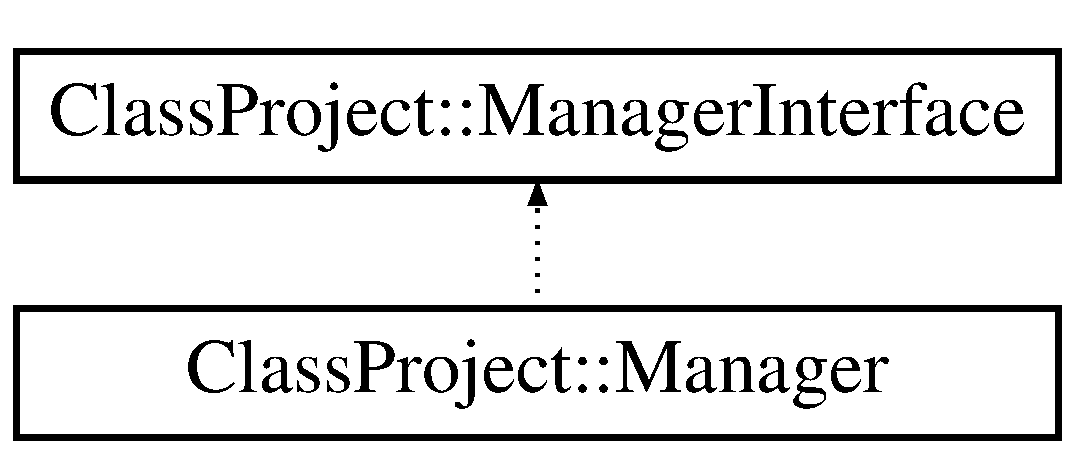
\includegraphics[height=2.000000cm]{classClassProject_1_1Manager}
\end{center}
\end{figure}
\subsection*{Public Member Functions}
\begin{DoxyCompactItemize}
\item 
{\bf Manager} ()
\begin{DoxyCompactList}\small\item\em \doxyref{Manager}{p.}{classClassProject_1_1Manager} Class. \end{DoxyCompactList}\item 
B\+D\+D\+\_\+\+ID {\bf create\+Var} (const std\+::string \&label) override
\begin{DoxyCompactList}\small\item\em Function to create a new Variable. \end{DoxyCompactList}\item 
const B\+D\+D\+\_\+\+ID \& {\bf True} () override
\begin{DoxyCompactList}\small\item\em Function to return the id of the T\+R\+UE leaf node in the Binary Tree. \end{DoxyCompactList}\item 
const B\+D\+D\+\_\+\+ID \& {\bf False} () override
\begin{DoxyCompactList}\small\item\em Function to return the id of the F\+A\+L\+SE leaf node in the Binary Tree. \end{DoxyCompactList}\item 
bool {\bf is\+Constant} (const B\+D\+D\+\_\+\+ID f) override
\begin{DoxyCompactList}\small\item\em Function to test if a given B\+D\+D\+\_\+\+ID is a Constant. \end{DoxyCompactList}\item 
bool {\bf is\+Variable} (const B\+D\+D\+\_\+\+ID x) override
\begin{DoxyCompactList}\small\item\em Function to test if a given B\+D\+D\+\_\+\+ID is a Variable. \end{DoxyCompactList}\item 
B\+D\+D\+\_\+\+ID {\bf top\+Var} (const B\+D\+D\+\_\+\+ID f) override
\begin{DoxyCompactList}\small\item\em Function to return the top variable of a given B\+D\+D\+\_\+\+ID. \end{DoxyCompactList}\item 
B\+D\+D\+\_\+\+ID {\bf ite} (const B\+D\+D\+\_\+\+ID i, const B\+D\+D\+\_\+\+ID t, const B\+D\+D\+\_\+\+ID e) override
\begin{DoxyCompactList}\small\item\em Function to compute the I\+F(\+B\+D\+D\+\_\+\+I\+D i) then(\+B\+D\+D\+\_\+\+I\+D t) E\+L\+S\+E(\+B\+D\+D\+\_\+\+I\+D e) Operator. \end{DoxyCompactList}\item 
B\+D\+D\+\_\+\+ID {\bf co\+Factor\+True} (const B\+D\+D\+\_\+\+ID f, B\+D\+D\+\_\+\+ID x) override
\begin{DoxyCompactList}\small\item\em Function to compute the T\+R\+UE co\+Factor of a given B\+D\+D\+\_\+\+ID f with respect to B\+D\+D\+\_\+\+ID x. \end{DoxyCompactList}\item 
B\+D\+D\+\_\+\+ID {\bf co\+Factor\+False} (const B\+D\+D\+\_\+\+ID f, B\+D\+D\+\_\+\+ID x) override
\begin{DoxyCompactList}\small\item\em Function to compute the F\+A\+L\+SE co\+Factor of a given B\+D\+D\+\_\+\+ID f with respect to B\+D\+D\+\_\+\+ID x. \end{DoxyCompactList}\item 
B\+D\+D\+\_\+\+ID {\bf co\+Factor\+True} (const B\+D\+D\+\_\+\+ID f) override
\begin{DoxyCompactList}\small\item\em Function to compute the T\+R\+UE co\+Factor of a given B\+D\+D\+\_\+\+ID f. \end{DoxyCompactList}\item 
B\+D\+D\+\_\+\+ID {\bf co\+Factor\+False} (const B\+D\+D\+\_\+\+ID f) override
\begin{DoxyCompactList}\small\item\em Function to compute the F\+A\+L\+SE co\+Factor of a given B\+D\+D\+\_\+\+ID f. \end{DoxyCompactList}\item 
B\+D\+D\+\_\+\+ID {\bf and2} (const B\+D\+D\+\_\+\+ID a, const B\+D\+D\+\_\+\+ID b) override
\begin{DoxyCompactList}\small\item\em Function to compute an A\+ND Boolean Function of two given B\+D\+D\+\_\+\+I\+Ds a and b. \end{DoxyCompactList}\item 
B\+D\+D\+\_\+\+ID {\bf or2} (const B\+D\+D\+\_\+\+ID a, const B\+D\+D\+\_\+\+ID b) override
\begin{DoxyCompactList}\small\item\em Function to compute an OR Boolean Function of two given B\+D\+D\+\_\+\+I\+Ds a and b. \end{DoxyCompactList}\item 
B\+D\+D\+\_\+\+ID {\bf xor2} (const B\+D\+D\+\_\+\+ID a, const B\+D\+D\+\_\+\+ID b) override
\begin{DoxyCompactList}\small\item\em Function to compute an X\+OR Boolean Function of two given B\+D\+D\+\_\+\+I\+Ds a and b. \end{DoxyCompactList}\item 
B\+D\+D\+\_\+\+ID {\bf neg} (const B\+D\+D\+\_\+\+ID a) override
\begin{DoxyCompactList}\small\item\em Function to compute the Negation of a given B\+D\+D\+\_\+\+ID. \end{DoxyCompactList}\item 
B\+D\+D\+\_\+\+ID {\bf nand2} (const B\+D\+D\+\_\+\+ID a, const B\+D\+D\+\_\+\+ID b) override
\begin{DoxyCompactList}\small\item\em Function to compute a N\+A\+ND Boolean Function of two given B\+D\+D\+\_\+\+I\+Ds a and b. \end{DoxyCompactList}\item 
B\+D\+D\+\_\+\+ID {\bf nor2} (const B\+D\+D\+\_\+\+ID a, const B\+D\+D\+\_\+\+ID b) override
\begin{DoxyCompactList}\small\item\em Function to compute a N\+OR Boolean Function of two given B\+D\+D\+\_\+\+I\+Ds a and b. \end{DoxyCompactList}\item 
std\+::string {\bf get\+Top\+Var\+Name} (const B\+D\+D\+\_\+\+ID \&root) override
\begin{DoxyCompactList}\small\item\em Function to get the name of the Top Variable of a given B\+D\+D\+\_\+\+ID. \end{DoxyCompactList}\item 
void {\bf find\+Nodes} (const B\+D\+D\+\_\+\+ID \&root, std\+::set$<$ B\+D\+D\+\_\+\+ID $>$ \&nodes\+\_\+of\+\_\+root) override
\begin{DoxyCompactList}\small\item\em Function to find out all the reachable nodes in the Binary Tree starting from a given B\+D\+D\+\_\+\+ID. \end{DoxyCompactList}\item 
void {\bf find\+Vars} (const B\+D\+D\+\_\+\+ID \&root, std\+::set$<$ B\+D\+D\+\_\+\+ID $>$ \&vars\+\_\+of\+\_\+root) override
\begin{DoxyCompactList}\small\item\em Function to find out all the reachable Variables in the Binary Tree starting from a given B\+D\+D\+\_\+\+ID. \end{DoxyCompactList}\item 
size\+\_\+t {\bf unique\+Table\+Size} () override
\begin{DoxyCompactList}\small\item\em Function to return the size of the unique\+Table. \end{DoxyCompactList}\item 
size\+\_\+t {\bf new\+Nodes\+Size} ()
\begin{DoxyCompactList}\small\item\em Function to return the size of the new\+\_\+nodes. \end{DoxyCompactList}\item 
size\+\_\+t {\bf computed\+Table\+Size} ()
\begin{DoxyCompactList}\small\item\em Function to return the size of the Computed Table. \end{DoxyCompactList}\item 
const {\bf B\+D\+D\+\_\+\+Node} \& {\bf get\+B\+D\+D\+Node} (B\+D\+D\+\_\+\+ID id)
\begin{DoxyCompactList}\small\item\em Function to return a \doxyref{B\+D\+D\+\_\+\+Node}{p.}{structClassProject_1_1BDD__Node} from the unique\+Table according to its B\+D\+D\+\_\+\+ID. \end{DoxyCompactList}\item 
void {\bf print\+Unique\+Table} ()\label{classClassProject_1_1Manager_afe9e70c59d3ee82369a9176fa53b20a6}

\begin{DoxyCompactList}\small\item\em Function to print all the B\+D\+D\+\_\+\+Nodes present in the unique\+Table, new\+\_\+nodes table and in the computed table. \end{DoxyCompactList}\end{DoxyCompactItemize}
\subsection*{Private Member Functions}
\begin{DoxyCompactItemize}
\item 
bool {\bf is\+Complement} (B\+D\+D\+\_\+\+ID f)
\begin{DoxyCompactList}\small\item\em Function check if a given B\+D\+D\+\_\+\+ID is a complement of a previous B\+D\+D\+\_\+\+ID. \end{DoxyCompactList}\item 
B\+D\+D\+\_\+\+ID {\bf get\+Complement} (B\+D\+D\+\_\+\+ID f)
\begin{DoxyCompactList}\small\item\em Function to return the coplement of a given B\+D\+D\+\_\+\+ID. \end{DoxyCompactList}\item 
B\+D\+D\+\_\+\+ID {\bf get\+Next\+Id} (B\+D\+D\+\_\+\+ID f)
\begin{DoxyCompactList}\small\item\em Function to get the next ID of a given B\+D\+D\+\_\+\+ID. \end{DoxyCompactList}\item 
B\+D\+D\+\_\+\+ID {\bf ite\+ST} (const B\+D\+D\+\_\+\+ID i, const B\+D\+D\+\_\+\+ID t, const B\+D\+D\+\_\+\+ID e)
\begin{DoxyCompactList}\small\item\em Function to compute the ite according to the standard triples. \end{DoxyCompactList}\item 
B\+D\+D\+\_\+\+ID {\bf ite} (const B\+D\+D\+\_\+\+ID i, const B\+D\+D\+\_\+\+ID t, const B\+D\+D\+\_\+\+ID e, const B\+D\+D\+\_\+\+ID top\+\_\+var)
\begin{DoxyCompactList}\small\item\em Function to compute the I\+F(\+B\+D\+D\+\_\+\+I\+D i) then(\+B\+D\+D\+\_\+\+I\+D t) E\+L\+S\+E(\+B\+D\+D\+\_\+\+I\+D e) Operator of a given B\+D\+D\+\_\+\+ID with respect to its top variable. \end{DoxyCompactList}\item 
B\+D\+D\+\_\+\+ID {\bf iteC} (const B\+D\+D\+\_\+\+ID i, const B\+D\+D\+\_\+\+ID t, const B\+D\+D\+\_\+\+ID e, const B\+D\+D\+\_\+\+ID top\+\_\+var)
\begin{DoxyCompactList}\small\item\em Function to compute the C\+O\+M\+P\+L\+E\+M\+E\+NT I\+F(\+B\+D\+D\+\_\+\+I\+D i) then(\+B\+D\+D\+\_\+\+I\+D t) E\+L\+S\+E(\+B\+D\+D\+\_\+\+I\+D e) Operator of a given B\+D\+D\+\_\+\+ID with respect to its top variable. \end{DoxyCompactList}\end{DoxyCompactItemize}
\subsection*{Private Attributes}
\begin{DoxyCompactItemize}
\item 
B\+D\+D\+\_\+\+ID {\bfseries false\+Node} = B\+D\+D\+\_\+\+I\+D\+\_\+\+F\+A\+L\+SE\label{classClassProject_1_1Manager_aa3b1a27b556d3983d07265337818cdc4}

\item 
B\+D\+D\+\_\+\+ID {\bfseries true\+Node} = B\+D\+D\+\_\+\+I\+D\+\_\+\+T\+R\+UE\label{classClassProject_1_1Manager_a81e5b193e33ce258286f1413ea1930d0}

\item 
vector$<$ {\bf B\+D\+D\+\_\+\+Node} $>$ {\bfseries unique\+\_\+table}\label{classClassProject_1_1Manager_acae2e50ceb565e95f1ee2a10199bf90b}

\item 
unordered\+\_\+map$<$ {\bf B\+D\+D\+\_\+\+Node}, B\+D\+D\+\_\+\+ID, {\bf B\+D\+D\+Hasher}, {\bf B\+D\+D\+Comparer} $>$ {\bf new\+\_\+nodes}
\item 
unordered\+\_\+map$<$ {\bf B\+D\+D\+\_\+\+Node}, B\+D\+D\+\_\+\+ID, {\bf B\+D\+D\+Hasher}, {\bf B\+D\+D\+Comparer} $>$ {\bf computed\+\_\+table}
\end{DoxyCompactItemize}


\subsection{Detailed Description}
\doxyref{Manager}{p.}{classClassProject_1_1Manager} Class. 

Declaration of the functions from the \doxyref{Manager\+Interface}{p.}{classClassProject_1_1ManagerInterface}. 

\subsection{Constructor \& Destructor Documentation}
\index{Class\+Project\+::\+Manager@{Class\+Project\+::\+Manager}!Manager@{Manager}}
\index{Manager@{Manager}!Class\+Project\+::\+Manager@{Class\+Project\+::\+Manager}}
\subsubsection[{Manager()}]{\setlength{\rightskip}{0pt plus 5cm}Manager\+::\+Manager (
\begin{DoxyParamCaption}
{}
\end{DoxyParamCaption}
)}\label{classClassProject_1_1Manager_a1658ff9f18e38ccd9cb8b0b371b9c20b}


\doxyref{Manager}{p.}{classClassProject_1_1Manager} Class. 

Implements the virtual functions from the Manager\+Interface.\+Manager Constructor. \doxyref{B\+D\+D\+\_\+\+Node}{p.}{structClassProject_1_1BDD__Node} true\+Node.

Initiates the T\+R\+UE leaf of node the Binary Tree. 

\subsection{Member Function Documentation}
\index{Class\+Project\+::\+Manager@{Class\+Project\+::\+Manager}!and2@{and2}}
\index{and2@{and2}!Class\+Project\+::\+Manager@{Class\+Project\+::\+Manager}}
\subsubsection[{and2(const B\+D\+D\+\_\+\+I\+D a, const B\+D\+D\+\_\+\+I\+D b) override}]{\setlength{\rightskip}{0pt plus 5cm}B\+D\+D\+\_\+\+ID Manager\+::and2 (
\begin{DoxyParamCaption}
\item[{const B\+D\+D\+\_\+\+ID}]{a, }
\item[{const B\+D\+D\+\_\+\+ID}]{b}
\end{DoxyParamCaption}
)\hspace{0.3cm}{\ttfamily [override]}, {\ttfamily [virtual]}}\label{classClassProject_1_1Manager_a75bd703f518ab88006bb2b493569ba08}


Function to compute an A\+ND Boolean Function of two given B\+D\+D\+\_\+\+I\+Ds a and b. 


\begin{DoxyParams}{Parameters}
{\em a} & a B\+D\+D\+\_\+\+ID argument. \\
\hline
{\em b} & a B\+D\+D\+\_\+\+ID argument.\+id \\
\hline
\end{DoxyParams}
\begin{DoxyReturn}{Returns}
Return the computed I\+TE operator of B\+D\+D\+\_\+\+I\+Ds a and b according to the A\+ND Function. 
\end{DoxyReturn}


Implements {\bf Class\+Project\+::\+Manager\+Interface} \doxyref{}{p.}{classClassProject_1_1ManagerInterface}.



References ite().

\index{Class\+Project\+::\+Manager@{Class\+Project\+::\+Manager}!co\+Factor\+False@{co\+Factor\+False}}
\index{co\+Factor\+False@{co\+Factor\+False}!Class\+Project\+::\+Manager@{Class\+Project\+::\+Manager}}
\subsubsection[{co\+Factor\+False(const B\+D\+D\+\_\+\+I\+D f, B\+D\+D\+\_\+\+I\+D x) override}]{\setlength{\rightskip}{0pt plus 5cm}B\+D\+D\+\_\+\+ID Manager\+::co\+Factor\+False (
\begin{DoxyParamCaption}
\item[{const B\+D\+D\+\_\+\+ID}]{f, }
\item[{B\+D\+D\+\_\+\+ID}]{x}
\end{DoxyParamCaption}
)\hspace{0.3cm}{\ttfamily [override]}, {\ttfamily [virtual]}}\label{classClassProject_1_1Manager_a91b0f680c53a9813e11f590f99c21264}


Function to compute the F\+A\+L\+SE co\+Factor of a given B\+D\+D\+\_\+\+ID f with respect to B\+D\+D\+\_\+\+ID x. 


\begin{DoxyParams}{Parameters}
{\em f} & a B\+D\+D\+\_\+\+ID argument. \\
\hline
{\em x} & a B\+D\+D\+\_\+\+ID argument. \\
\hline
\end{DoxyParams}
\begin{DoxyReturn}{Returns}
Return the computed I\+TE operator of the T\+R\+UE, and F\+A\+L\+SE branches of B\+D\+D\+\_\+\+ID f with respect to B\+D\+D\+\_\+\+ID x. 
\end{DoxyReturn}


Implements {\bf Class\+Project\+::\+Manager\+Interface} \doxyref{}{p.}{classClassProject_1_1ManagerInterface}.



References co\+Factor\+True(), get\+Complement(), is\+Complement(), is\+Constant(), ite(), and top\+Var().



Referenced by co\+Factor\+True(), find\+Nodes(), find\+Vars(), ite(), and ite\+C().

\index{Class\+Project\+::\+Manager@{Class\+Project\+::\+Manager}!co\+Factor\+False@{co\+Factor\+False}}
\index{co\+Factor\+False@{co\+Factor\+False}!Class\+Project\+::\+Manager@{Class\+Project\+::\+Manager}}
\subsubsection[{co\+Factor\+False(const B\+D\+D\+\_\+\+I\+D f) override}]{\setlength{\rightskip}{0pt plus 5cm}B\+D\+D\+\_\+\+ID Manager\+::co\+Factor\+False (
\begin{DoxyParamCaption}
\item[{const B\+D\+D\+\_\+\+ID}]{f}
\end{DoxyParamCaption}
)\hspace{0.3cm}{\ttfamily [override]}, {\ttfamily [virtual]}}\label{classClassProject_1_1Manager_ac9621e396f35aebfefa623a5c67e32a1}


Function to compute the F\+A\+L\+SE co\+Factor of a given B\+D\+D\+\_\+\+ID f. 


\begin{DoxyParams}{Parameters}
{\em f} & a B\+D\+D\+\_\+\+ID argument. \\
\hline
\end{DoxyParams}
\begin{DoxyReturn}{Returns}
Return the F\+A\+L\+SE co\+Factor of the given B\+D\+D\+\_\+\+ID f. 
\end{DoxyReturn}


Implements {\bf Class\+Project\+::\+Manager\+Interface} \doxyref{}{p.}{classClassProject_1_1ManagerInterface}.



References get\+B\+D\+D\+Node(), and Class\+Project\+::\+B\+D\+D\+\_\+\+Node\+::low.

\index{Class\+Project\+::\+Manager@{Class\+Project\+::\+Manager}!co\+Factor\+True@{co\+Factor\+True}}
\index{co\+Factor\+True@{co\+Factor\+True}!Class\+Project\+::\+Manager@{Class\+Project\+::\+Manager}}
\subsubsection[{co\+Factor\+True(const B\+D\+D\+\_\+\+I\+D f, B\+D\+D\+\_\+\+I\+D x) override}]{\setlength{\rightskip}{0pt plus 5cm}B\+D\+D\+\_\+\+ID Manager\+::co\+Factor\+True (
\begin{DoxyParamCaption}
\item[{const B\+D\+D\+\_\+\+ID}]{f, }
\item[{B\+D\+D\+\_\+\+ID}]{x}
\end{DoxyParamCaption}
)\hspace{0.3cm}{\ttfamily [override]}, {\ttfamily [virtual]}}\label{classClassProject_1_1Manager_ae58b05ca4ddd764390db56a1e22e7b07}


Function to compute the T\+R\+UE co\+Factor of a given B\+D\+D\+\_\+\+ID f with respect to B\+D\+D\+\_\+\+ID x. 


\begin{DoxyParams}{Parameters}
{\em f} & a B\+D\+D\+\_\+\+ID argument. \\
\hline
{\em x} & a B\+D\+D\+\_\+\+ID argument. \\
\hline
\end{DoxyParams}
\begin{DoxyReturn}{Returns}
Return the computed I\+TE operator of the T\+R\+UE, and F\+A\+L\+SE branches of B\+D\+D\+\_\+\+ID f with respect to B\+D\+D\+\_\+\+ID x. 
\end{DoxyReturn}


Implements {\bf Class\+Project\+::\+Manager\+Interface} \doxyref{}{p.}{classClassProject_1_1ManagerInterface}.



References co\+Factor\+False(), get\+Complement(), is\+Complement(), is\+Constant(), ite(), and top\+Var().



Referenced by co\+Factor\+False(), find\+Nodes(), find\+Vars(), ite(), and ite\+C().

\index{Class\+Project\+::\+Manager@{Class\+Project\+::\+Manager}!co\+Factor\+True@{co\+Factor\+True}}
\index{co\+Factor\+True@{co\+Factor\+True}!Class\+Project\+::\+Manager@{Class\+Project\+::\+Manager}}
\subsubsection[{co\+Factor\+True(const B\+D\+D\+\_\+\+I\+D f) override}]{\setlength{\rightskip}{0pt plus 5cm}B\+D\+D\+\_\+\+ID Manager\+::co\+Factor\+True (
\begin{DoxyParamCaption}
\item[{const B\+D\+D\+\_\+\+ID}]{f}
\end{DoxyParamCaption}
)\hspace{0.3cm}{\ttfamily [override]}, {\ttfamily [virtual]}}\label{classClassProject_1_1Manager_abc6417257171d6032a7dee6ea2ecd8d3}


Function to compute the T\+R\+UE co\+Factor of a given B\+D\+D\+\_\+\+ID f. 


\begin{DoxyParams}{Parameters}
{\em f} & a B\+D\+D\+\_\+\+ID argument. \\
\hline
\end{DoxyParams}
\begin{DoxyReturn}{Returns}
Return the T\+R\+UE co\+Factor of the given B\+D\+D\+\_\+\+ID f. 
\end{DoxyReturn}


Implements {\bf Class\+Project\+::\+Manager\+Interface} \doxyref{}{p.}{classClassProject_1_1ManagerInterface}.



References get\+B\+D\+D\+Node(), and Class\+Project\+::\+B\+D\+D\+\_\+\+Node\+::high.

\index{Class\+Project\+::\+Manager@{Class\+Project\+::\+Manager}!computed\+Table\+Size@{computed\+Table\+Size}}
\index{computed\+Table\+Size@{computed\+Table\+Size}!Class\+Project\+::\+Manager@{Class\+Project\+::\+Manager}}
\subsubsection[{computed\+Table\+Size()}]{\setlength{\rightskip}{0pt plus 5cm}size\+\_\+t Manager\+::computed\+Table\+Size (
\begin{DoxyParamCaption}
{}
\end{DoxyParamCaption}
)}\label{classClassProject_1_1Manager_a6fa41070bf454641df27e9d4dfd30ce4}


Function to return the size of the Computed Table. 

\begin{DoxyReturn}{Returns}
the size of computed\+\_\+table. 
\end{DoxyReturn}


References computed\+\_\+table.

\index{Class\+Project\+::\+Manager@{Class\+Project\+::\+Manager}!create\+Var@{create\+Var}}
\index{create\+Var@{create\+Var}!Class\+Project\+::\+Manager@{Class\+Project\+::\+Manager}}
\subsubsection[{create\+Var(const std\+::string \&label) override}]{\setlength{\rightskip}{0pt plus 5cm}B\+D\+D\+\_\+\+ID Manager\+::create\+Var (
\begin{DoxyParamCaption}
\item[{const std\+::string \&}]{label}
\end{DoxyParamCaption}
)\hspace{0.3cm}{\ttfamily [override]}, {\ttfamily [virtual]}}\label{classClassProject_1_1Manager_aa3fe08b0b002032a13a5ff9d05f39cfd}


Function to create a new Variable. 


\begin{DoxyParams}{Parameters}
{\em label} & a string argument. \\
\hline
\end{DoxyParams}
\begin{DoxyReturn}{Returns}
The id of the new variable which correspond to the size of the unique\+Table. 
\end{DoxyReturn}
B\+D\+D\+\_\+\+ID value id.

\doxyref{B\+D\+D\+\_\+\+Node}{p.}{structClassProject_1_1BDD__Node} value var. 

Implements {\bf Class\+Project\+::\+Manager\+Interface} \doxyref{}{p.}{classClassProject_1_1ManagerInterface}.

\index{Class\+Project\+::\+Manager@{Class\+Project\+::\+Manager}!False@{False}}
\index{False@{False}!Class\+Project\+::\+Manager@{Class\+Project\+::\+Manager}}
\subsubsection[{False() override}]{\setlength{\rightskip}{0pt plus 5cm}const B\+D\+D\+\_\+\+ID \& Manager\+::\+False (
\begin{DoxyParamCaption}
{}
\end{DoxyParamCaption}
)\hspace{0.3cm}{\ttfamily [override]}, {\ttfamily [virtual]}}\label{classClassProject_1_1Manager_a699638a290747c865312b4c130260a06}


Function to return the id of the F\+A\+L\+SE leaf node in the Binary Tree. 

\begin{DoxyReturn}{Returns}
The id of the False leaf node in the Binary Tree. 
\end{DoxyReturn}


Implements {\bf Class\+Project\+::\+Manager\+Interface} \doxyref{}{p.}{classClassProject_1_1ManagerInterface}.

\index{Class\+Project\+::\+Manager@{Class\+Project\+::\+Manager}!find\+Nodes@{find\+Nodes}}
\index{find\+Nodes@{find\+Nodes}!Class\+Project\+::\+Manager@{Class\+Project\+::\+Manager}}
\subsubsection[{find\+Nodes(const B\+D\+D\+\_\+\+I\+D \&root, std\+::set$<$ B\+D\+D\+\_\+\+I\+D $>$ \&nodes\+\_\+of\+\_\+root) override}]{\setlength{\rightskip}{0pt plus 5cm}void Manager\+::find\+Nodes (
\begin{DoxyParamCaption}
\item[{const B\+D\+D\+\_\+\+ID \&}]{root, }
\item[{std\+::set$<$ B\+D\+D\+\_\+\+ID $>$ \&}]{nodes\+\_\+of\+\_\+root}
\end{DoxyParamCaption}
)\hspace{0.3cm}{\ttfamily [override]}, {\ttfamily [virtual]}}\label{classClassProject_1_1Manager_a9d465fdff670b0bd9ef4a35ab9611f25}


Function to find out all the reachable nodes in the Binary Tree starting from a given B\+D\+D\+\_\+\+ID. 


\begin{DoxyParams}{Parameters}
{\em root} & a B\+D\+D\+\_\+\+ID argument. \\
\hline
\end{DoxyParams}
\begin{DoxyReturn}{Returns}
Return set containing all the reachable Nodes from a given Node. 
\end{DoxyReturn}


Implements {\bf Class\+Project\+::\+Manager\+Interface} \doxyref{}{p.}{classClassProject_1_1ManagerInterface}.



References co\+Factor\+False(), co\+Factor\+True(), and is\+Constant().

\index{Class\+Project\+::\+Manager@{Class\+Project\+::\+Manager}!find\+Vars@{find\+Vars}}
\index{find\+Vars@{find\+Vars}!Class\+Project\+::\+Manager@{Class\+Project\+::\+Manager}}
\subsubsection[{find\+Vars(const B\+D\+D\+\_\+\+I\+D \&root, std\+::set$<$ B\+D\+D\+\_\+\+I\+D $>$ \&vars\+\_\+of\+\_\+root) override}]{\setlength{\rightskip}{0pt plus 5cm}void Manager\+::find\+Vars (
\begin{DoxyParamCaption}
\item[{const B\+D\+D\+\_\+\+ID \&}]{root, }
\item[{std\+::set$<$ B\+D\+D\+\_\+\+ID $>$ \&}]{vars\+\_\+of\+\_\+root}
\end{DoxyParamCaption}
)\hspace{0.3cm}{\ttfamily [override]}, {\ttfamily [virtual]}}\label{classClassProject_1_1Manager_a759513c0bb7447bfb05a82a818ab22eb}


Function to find out all the reachable Variables in the Binary Tree starting from a given B\+D\+D\+\_\+\+ID. 


\begin{DoxyParams}{Parameters}
{\em root} & a B\+D\+D\+\_\+\+ID argument. \\
\hline
\end{DoxyParams}
\begin{DoxyReturn}{Returns}
Return set containing all the reachable Variables from a given Node. 
\end{DoxyReturn}


Implements {\bf Class\+Project\+::\+Manager\+Interface} \doxyref{}{p.}{classClassProject_1_1ManagerInterface}.



References co\+Factor\+False(), co\+Factor\+True(), is\+Constant(), and top\+Var().

\index{Class\+Project\+::\+Manager@{Class\+Project\+::\+Manager}!get\+B\+D\+D\+Node@{get\+B\+D\+D\+Node}}
\index{get\+B\+D\+D\+Node@{get\+B\+D\+D\+Node}!Class\+Project\+::\+Manager@{Class\+Project\+::\+Manager}}
\subsubsection[{get\+B\+D\+D\+Node(\+B\+D\+D\+\_\+\+I\+D id)}]{\setlength{\rightskip}{0pt plus 5cm}const {\bf B\+D\+D\+\_\+\+Node} \& Manager\+::get\+B\+D\+D\+Node (
\begin{DoxyParamCaption}
\item[{B\+D\+D\+\_\+\+ID}]{id}
\end{DoxyParamCaption}
)}\label{classClassProject_1_1Manager_a8b72bfe987f1b424c42141172defa321}


Function to return a \doxyref{B\+D\+D\+\_\+\+Node}{p.}{structClassProject_1_1BDD__Node} from the unique\+Table according to its B\+D\+D\+\_\+\+ID. 


\begin{DoxyParams}{Parameters}
{\em id} & a B\+D\+D\+\_\+\+ID argument. \\
\hline
\end{DoxyParams}
\begin{DoxyReturn}{Returns}
Return a \doxyref{B\+D\+D\+\_\+\+Node}{p.}{structClassProject_1_1BDD__Node} from the unique\+Table that has the corresponding B\+D\+D\+\_\+\+ID. 
\end{DoxyReturn}


References is\+Constant().



Referenced by co\+Factor\+False(), co\+Factor\+True(), get\+Top\+Var\+Name(), is\+Variable(), and top\+Var().

\index{Class\+Project\+::\+Manager@{Class\+Project\+::\+Manager}!get\+Complement@{get\+Complement}}
\index{get\+Complement@{get\+Complement}!Class\+Project\+::\+Manager@{Class\+Project\+::\+Manager}}
\subsubsection[{get\+Complement(\+B\+D\+D\+\_\+\+I\+D f)}]{\setlength{\rightskip}{0pt plus 5cm}B\+D\+D\+\_\+\+ID Manager\+::get\+Complement (
\begin{DoxyParamCaption}
\item[{B\+D\+D\+\_\+\+ID}]{f}
\end{DoxyParamCaption}
)\hspace{0.3cm}{\ttfamily [private]}}\label{classClassProject_1_1Manager_a11656a3ce5a4ba0e71a65ac874d89813}


Function to return the coplement of a given B\+D\+D\+\_\+\+ID. 


\begin{DoxyParams}{Parameters}
{\em f} & a B\+D\+D\+\_\+\+ID argument. \\
\hline
\end{DoxyParams}
\begin{DoxyReturn}{Returns}
B\+D\+D\+\_\+\+I\+D\+\_\+\+T\+R\+UE or F\+A\+L\+SE if f is a constant, otherwise return the B\+D\+D\+\_\+\+ID of f +1 if B\+D\+D\+\_\+\+ID is even, or B\+D\+D\+\_\+\+ID -\/1 if it\textquotesingle{}s odd. 
\end{DoxyReturn}


References is\+Constant().



Referenced by co\+Factor\+False(), co\+Factor\+True(), ite(), ite\+C(), and ite\+S\+T().

\index{Class\+Project\+::\+Manager@{Class\+Project\+::\+Manager}!get\+Next\+Id@{get\+Next\+Id}}
\index{get\+Next\+Id@{get\+Next\+Id}!Class\+Project\+::\+Manager@{Class\+Project\+::\+Manager}}
\subsubsection[{get\+Next\+Id(\+B\+D\+D\+\_\+\+I\+D f)}]{\setlength{\rightskip}{0pt plus 5cm}B\+D\+D\+\_\+\+ID Manager\+::get\+Next\+Id (
\begin{DoxyParamCaption}
\item[{B\+D\+D\+\_\+\+ID}]{f}
\end{DoxyParamCaption}
)\hspace{0.3cm}{\ttfamily [private]}}\label{classClassProject_1_1Manager_a0baa1de7f305b8a6d972784c3399ee73}


Function to get the next ID of a given B\+D\+D\+\_\+\+ID. 


\begin{DoxyParams}{Parameters}
{\em f} & a B\+D\+D\+\_\+\+ID argument. \\
\hline
\end{DoxyParams}
\begin{DoxyReturn}{Returns}
the next B\+D\+D\+\_\+\+ID of f. 
\end{DoxyReturn}


References is\+Complement().



Referenced by ite\+S\+T().

\index{Class\+Project\+::\+Manager@{Class\+Project\+::\+Manager}!get\+Top\+Var\+Name@{get\+Top\+Var\+Name}}
\index{get\+Top\+Var\+Name@{get\+Top\+Var\+Name}!Class\+Project\+::\+Manager@{Class\+Project\+::\+Manager}}
\subsubsection[{get\+Top\+Var\+Name(const B\+D\+D\+\_\+\+I\+D \&root) override}]{\setlength{\rightskip}{0pt plus 5cm}std\+::string Manager\+::get\+Top\+Var\+Name (
\begin{DoxyParamCaption}
\item[{const B\+D\+D\+\_\+\+ID \&}]{root}
\end{DoxyParamCaption}
)\hspace{0.3cm}{\ttfamily [override]}, {\ttfamily [virtual]}}\label{classClassProject_1_1Manager_a7238da7832b931611dbfd273800360e2}


Function to get the name of the Top Variable of a given B\+D\+D\+\_\+\+ID. 


\begin{DoxyParams}{Parameters}
{\em root} & a B\+D\+D\+\_\+\+ID argument. \\
\hline
\end{DoxyParams}
\begin{DoxyReturn}{Returns}
Return the label(\+Top Varaible Name) of the given B\+D\+D\+\_\+\+ID root. 
\end{DoxyReturn}


Implements {\bf Class\+Project\+::\+Manager\+Interface} \doxyref{}{p.}{classClassProject_1_1ManagerInterface}.



References get\+B\+D\+D\+Node().

\index{Class\+Project\+::\+Manager@{Class\+Project\+::\+Manager}!is\+Complement@{is\+Complement}}
\index{is\+Complement@{is\+Complement}!Class\+Project\+::\+Manager@{Class\+Project\+::\+Manager}}
\subsubsection[{is\+Complement(\+B\+D\+D\+\_\+\+I\+D f)}]{\setlength{\rightskip}{0pt plus 5cm}bool Manager\+::is\+Complement (
\begin{DoxyParamCaption}
\item[{B\+D\+D\+\_\+\+ID}]{f}
\end{DoxyParamCaption}
)\hspace{0.3cm}{\ttfamily [private]}}\label{classClassProject_1_1Manager_a5e47cffe40b3f094fb29715526740f50}


Function check if a given B\+D\+D\+\_\+\+ID is a complement of a previous B\+D\+D\+\_\+\+ID. 

Table that contains the computed ite calculations in order to eliminate reptition on the computations.


\begin{DoxyParams}{Parameters}
{\em f} & a B\+D\+D\+\_\+\+ID argument. \\
\hline
\end{DoxyParams}
\begin{DoxyReturn}{Returns}
T\+R\+UE in the case of f be a complent B\+D\+D\+\_\+\+ID, otherwise return F\+A\+L\+SE. 
\end{DoxyReturn}


References is\+Constant().



Referenced by co\+Factor\+False(), co\+Factor\+True(), get\+Next\+Id(), and ite().

\index{Class\+Project\+::\+Manager@{Class\+Project\+::\+Manager}!is\+Constant@{is\+Constant}}
\index{is\+Constant@{is\+Constant}!Class\+Project\+::\+Manager@{Class\+Project\+::\+Manager}}
\subsubsection[{is\+Constant(const B\+D\+D\+\_\+\+I\+D f) override}]{\setlength{\rightskip}{0pt plus 5cm}bool Manager\+::is\+Constant (
\begin{DoxyParamCaption}
\item[{const B\+D\+D\+\_\+\+ID}]{f}
\end{DoxyParamCaption}
)\hspace{0.3cm}{\ttfamily [override]}, {\ttfamily [virtual]}}\label{classClassProject_1_1Manager_a13edef310f5e0ea718619151a7be451a}


Function to test if a given B\+D\+D\+\_\+\+ID is a Constant. 


\begin{DoxyParams}{Parameters}
{\em f} & a B\+D\+D\+\_\+\+ID argument. \\
\hline
\end{DoxyParams}
\begin{DoxyReturn}{Returns}
T\+R\+UE in case that the given B\+D\+D\+\_\+\+ID f is a Constant, otherwise return F\+A\+L\+SE. 
\end{DoxyReturn}


Implements {\bf Class\+Project\+::\+Manager\+Interface} \doxyref{}{p.}{classClassProject_1_1ManagerInterface}.



Referenced by co\+Factor\+False(), co\+Factor\+True(), find\+Nodes(), find\+Vars(), get\+B\+D\+D\+Node(), get\+Complement(), is\+Complement(), is\+Variable(), ite(), and ite\+S\+T().

\index{Class\+Project\+::\+Manager@{Class\+Project\+::\+Manager}!is\+Variable@{is\+Variable}}
\index{is\+Variable@{is\+Variable}!Class\+Project\+::\+Manager@{Class\+Project\+::\+Manager}}
\subsubsection[{is\+Variable(const B\+D\+D\+\_\+\+I\+D x) override}]{\setlength{\rightskip}{0pt plus 5cm}bool Manager\+::is\+Variable (
\begin{DoxyParamCaption}
\item[{const B\+D\+D\+\_\+\+ID}]{x}
\end{DoxyParamCaption}
)\hspace{0.3cm}{\ttfamily [override]}, {\ttfamily [virtual]}}\label{classClassProject_1_1Manager_a84c7144dc3c74e39dfb50a053da626a0}


Function to test if a given B\+D\+D\+\_\+\+ID is a Variable. 


\begin{DoxyParams}{Parameters}
{\em x} & a B\+D\+D\+\_\+\+ID argument. \\
\hline
\end{DoxyParams}
\begin{DoxyReturn}{Returns}
T\+R\+UE in case that the given B\+D\+D\+\_\+\+ID x is a Variable, otherwise return F\+A\+L\+SE. 
\end{DoxyReturn}
$<$ \doxyref{B\+D\+D\+\_\+\+Node}{p.}{structClassProject_1_1BDD__Node} pointer value node. 

Implements {\bf Class\+Project\+::\+Manager\+Interface} \doxyref{}{p.}{classClassProject_1_1ManagerInterface}.



References get\+B\+D\+D\+Node(), is\+Constant(), and Class\+Project\+::\+B\+D\+D\+\_\+\+Node\+::top\+\_\+var.

\index{Class\+Project\+::\+Manager@{Class\+Project\+::\+Manager}!ite@{ite}}
\index{ite@{ite}!Class\+Project\+::\+Manager@{Class\+Project\+::\+Manager}}
\subsubsection[{ite(const B\+D\+D\+\_\+\+I\+D i, const B\+D\+D\+\_\+\+I\+D t, const B\+D\+D\+\_\+\+I\+D e, const B\+D\+D\+\_\+\+I\+D top\+\_\+var)}]{\setlength{\rightskip}{0pt plus 5cm}B\+D\+D\+\_\+\+ID Manager\+::ite (
\begin{DoxyParamCaption}
\item[{const B\+D\+D\+\_\+\+ID}]{i, }
\item[{const B\+D\+D\+\_\+\+ID}]{t, }
\item[{const B\+D\+D\+\_\+\+ID}]{e, }
\item[{const B\+D\+D\+\_\+\+ID}]{top\+\_\+var}
\end{DoxyParamCaption}
)\hspace{0.3cm}{\ttfamily [private]}}\label{classClassProject_1_1Manager_a12f754fae1fd3b2322cf5dcd2eec095f}


Function to compute the I\+F(\+B\+D\+D\+\_\+\+I\+D i) then(\+B\+D\+D\+\_\+\+I\+D t) E\+L\+S\+E(\+B\+D\+D\+\_\+\+I\+D e) Operator of a given B\+D\+D\+\_\+\+ID with respect to its top variable. 


\begin{DoxyParams}{Parameters}
{\em i} & a B\+D\+D\+\_\+\+ID argument. \\
\hline
{\em t} & a B\+D\+D\+\_\+\+ID argument. \\
\hline
{\em e} & a B\+D\+D\+\_\+\+ID argument. \\
\hline
{\em top\+\_\+var} & a B\+D\+D\+\_\+\+ID argument. \\
\hline
\end{DoxyParams}
\begin{DoxyReturn}{Returns}
Return the id of the computed IF then E\+L\+SE Operator. 
\end{DoxyReturn}


References co\+Factor\+False(), co\+Factor\+True(), computed\+\_\+table, get\+Complement(), is\+Complement(), ite\+C(), new\+\_\+nodes, and unique\+Table\+Size().



Referenced by and2(), co\+Factor\+False(), co\+Factor\+True(), ite(), ite\+C(), ite\+S\+T(), nand2(), neg(), nor2(), or2(), and xor2().

\index{Class\+Project\+::\+Manager@{Class\+Project\+::\+Manager}!ite@{ite}}
\index{ite@{ite}!Class\+Project\+::\+Manager@{Class\+Project\+::\+Manager}}
\subsubsection[{ite(const B\+D\+D\+\_\+\+I\+D i, const B\+D\+D\+\_\+\+I\+D t, const B\+D\+D\+\_\+\+I\+D e) override}]{\setlength{\rightskip}{0pt plus 5cm}B\+D\+D\+\_\+\+ID Manager\+::ite (
\begin{DoxyParamCaption}
\item[{const B\+D\+D\+\_\+\+ID}]{i, }
\item[{const B\+D\+D\+\_\+\+ID}]{t, }
\item[{const B\+D\+D\+\_\+\+ID}]{e}
\end{DoxyParamCaption}
)\hspace{0.3cm}{\ttfamily [override]}, {\ttfamily [virtual]}}\label{classClassProject_1_1Manager_a615943b56ed99f812d4117ebb5bbc455}


Function to compute the I\+F(\+B\+D\+D\+\_\+\+I\+D i) then(\+B\+D\+D\+\_\+\+I\+D t) E\+L\+S\+E(\+B\+D\+D\+\_\+\+I\+D e) Operator. 


\begin{DoxyParams}{Parameters}
{\em i} & a B\+D\+D\+\_\+\+ID argument. \\
\hline
{\em t} & a B\+D\+D\+\_\+\+ID argument. \\
\hline
{\em e} & a B\+D\+D\+\_\+\+ID argument. \\
\hline
\end{DoxyParams}
\begin{DoxyReturn}{Returns}
Return the id of the computed IF then E\+L\+SE Operator. 
\end{DoxyReturn}


Implements {\bf Class\+Project\+::\+Manager\+Interface} \doxyref{}{p.}{classClassProject_1_1ManagerInterface}.



References get\+Complement(), is\+Constant(), ite(), ite\+S\+T(), and top\+Var().

\index{Class\+Project\+::\+Manager@{Class\+Project\+::\+Manager}!iteC@{iteC}}
\index{iteC@{iteC}!Class\+Project\+::\+Manager@{Class\+Project\+::\+Manager}}
\subsubsection[{ite\+C(const B\+D\+D\+\_\+\+I\+D i, const B\+D\+D\+\_\+\+I\+D t, const B\+D\+D\+\_\+\+I\+D e, const B\+D\+D\+\_\+\+I\+D top\+\_\+var)}]{\setlength{\rightskip}{0pt plus 5cm}B\+D\+D\+\_\+\+ID Manager\+::iteC (
\begin{DoxyParamCaption}
\item[{const B\+D\+D\+\_\+\+ID}]{i, }
\item[{const B\+D\+D\+\_\+\+ID}]{t, }
\item[{const B\+D\+D\+\_\+\+ID}]{e, }
\item[{const B\+D\+D\+\_\+\+ID}]{top\+\_\+var}
\end{DoxyParamCaption}
)\hspace{0.3cm}{\ttfamily [private]}}\label{classClassProject_1_1Manager_a60bfd3e2c706f5b7d96f3739aefd30fd}


Function to compute the C\+O\+M\+P\+L\+E\+M\+E\+NT I\+F(\+B\+D\+D\+\_\+\+I\+D i) then(\+B\+D\+D\+\_\+\+I\+D t) E\+L\+S\+E(\+B\+D\+D\+\_\+\+I\+D e) Operator of a given B\+D\+D\+\_\+\+ID with respect to its top variable. 


\begin{DoxyParams}{Parameters}
{\em i} & a B\+D\+D\+\_\+\+ID argument. \\
\hline
{\em t} & a B\+D\+D\+\_\+\+ID argument. \\
\hline
{\em e} & a B\+D\+D\+\_\+\+ID argument. \\
\hline
{\em top\+\_\+var} & a B\+D\+D\+\_\+\+ID argument. \\
\hline
\end{DoxyParams}
\begin{DoxyReturn}{Returns}
Return the id of the computed IF then E\+L\+SE Operator. 
\end{DoxyReturn}


References co\+Factor\+False(), co\+Factor\+True(), computed\+\_\+table, get\+Complement(), ite(), new\+\_\+nodes, and unique\+Table\+Size().



Referenced by ite().

\index{Class\+Project\+::\+Manager@{Class\+Project\+::\+Manager}!ite\+ST@{ite\+ST}}
\index{ite\+ST@{ite\+ST}!Class\+Project\+::\+Manager@{Class\+Project\+::\+Manager}}
\subsubsection[{ite\+S\+T(const B\+D\+D\+\_\+\+I\+D i, const B\+D\+D\+\_\+\+I\+D t, const B\+D\+D\+\_\+\+I\+D e)}]{\setlength{\rightskip}{0pt plus 5cm}B\+D\+D\+\_\+\+ID Manager\+::ite\+ST (
\begin{DoxyParamCaption}
\item[{const B\+D\+D\+\_\+\+ID}]{i, }
\item[{const B\+D\+D\+\_\+\+ID}]{t, }
\item[{const B\+D\+D\+\_\+\+ID}]{e}
\end{DoxyParamCaption}
)\hspace{0.3cm}{\ttfamily [private]}}\label{classClassProject_1_1Manager_a6c82345b580058836d1cd8a1c09399b6}


Function to compute the ite according to the standard triples. 


\begin{DoxyParams}{Parameters}
{\em i} & a B\+D\+D\+\_\+\+ID argument. \\
\hline
{\em t} & a B\+D\+D\+\_\+\+ID argument. \\
\hline
{\em e} & a B\+D\+D\+\_\+\+ID argument. \\
\hline
\end{DoxyParams}
\begin{DoxyReturn}{Returns}
the ID of the computed IF T\+H\+EN E\+L\+SE operator according to the standard triples. 
\end{DoxyReturn}


References get\+Complement(), get\+Next\+Id(), is\+Constant(), ite(), and top\+Var().



Referenced by ite().

\index{Class\+Project\+::\+Manager@{Class\+Project\+::\+Manager}!nand2@{nand2}}
\index{nand2@{nand2}!Class\+Project\+::\+Manager@{Class\+Project\+::\+Manager}}
\subsubsection[{nand2(const B\+D\+D\+\_\+\+I\+D a, const B\+D\+D\+\_\+\+I\+D b) override}]{\setlength{\rightskip}{0pt plus 5cm}B\+D\+D\+\_\+\+ID Manager\+::nand2 (
\begin{DoxyParamCaption}
\item[{const B\+D\+D\+\_\+\+ID}]{a, }
\item[{const B\+D\+D\+\_\+\+ID}]{b}
\end{DoxyParamCaption}
)\hspace{0.3cm}{\ttfamily [override]}, {\ttfamily [virtual]}}\label{classClassProject_1_1Manager_a94abdd8d633d6e52a052838305f97f36}


Function to compute a N\+A\+ND Boolean Function of two given B\+D\+D\+\_\+\+I\+Ds a and b. 


\begin{DoxyParams}{Parameters}
{\em a} & a B\+D\+D\+\_\+\+ID argument. \\
\hline
{\em b} & a B\+D\+D\+\_\+\+ID argument. \\
\hline
\end{DoxyParams}
\begin{DoxyReturn}{Returns}
Return the computed I\+TE operator of B\+D\+D\+\_\+\+I\+Ds a and b according to the N\+A\+ND Function. 
\end{DoxyReturn}


Implements {\bf Class\+Project\+::\+Manager\+Interface} \doxyref{}{p.}{classClassProject_1_1ManagerInterface}.



References ite(), and neg().

\index{Class\+Project\+::\+Manager@{Class\+Project\+::\+Manager}!neg@{neg}}
\index{neg@{neg}!Class\+Project\+::\+Manager@{Class\+Project\+::\+Manager}}
\subsubsection[{neg(const B\+D\+D\+\_\+\+I\+D a) override}]{\setlength{\rightskip}{0pt plus 5cm}B\+D\+D\+\_\+\+ID Manager\+::neg (
\begin{DoxyParamCaption}
\item[{const B\+D\+D\+\_\+\+ID}]{a}
\end{DoxyParamCaption}
)\hspace{0.3cm}{\ttfamily [override]}, {\ttfamily [virtual]}}\label{classClassProject_1_1Manager_a6c83a83001023096dd68183f40ee80b3}


Function to compute the Negation of a given B\+D\+D\+\_\+\+ID. 


\begin{DoxyParams}{Parameters}
{\em a} & a B\+D\+D\+\_\+\+ID argument. \\
\hline
\end{DoxyParams}
\begin{DoxyReturn}{Returns}
Return the Negation of a given B\+D\+D\+\_\+\+ID. 
\end{DoxyReturn}


Implements {\bf Class\+Project\+::\+Manager\+Interface} \doxyref{}{p.}{classClassProject_1_1ManagerInterface}.



References ite().



Referenced by nand2(), nor2(), and xor2().

\index{Class\+Project\+::\+Manager@{Class\+Project\+::\+Manager}!new\+Nodes\+Size@{new\+Nodes\+Size}}
\index{new\+Nodes\+Size@{new\+Nodes\+Size}!Class\+Project\+::\+Manager@{Class\+Project\+::\+Manager}}
\subsubsection[{new\+Nodes\+Size()}]{\setlength{\rightskip}{0pt plus 5cm}size\+\_\+t Manager\+::new\+Nodes\+Size (
\begin{DoxyParamCaption}
{}
\end{DoxyParamCaption}
)}\label{classClassProject_1_1Manager_a6a1039bfd40a5b78c8d7dc992815e5ec}


Function to return the size of the new\+\_\+nodes. 

\begin{DoxyReturn}{Returns}
the size of new\+\_\+nodes. 
\end{DoxyReturn}


References new\+\_\+nodes.

\index{Class\+Project\+::\+Manager@{Class\+Project\+::\+Manager}!nor2@{nor2}}
\index{nor2@{nor2}!Class\+Project\+::\+Manager@{Class\+Project\+::\+Manager}}
\subsubsection[{nor2(const B\+D\+D\+\_\+\+I\+D a, const B\+D\+D\+\_\+\+I\+D b) override}]{\setlength{\rightskip}{0pt plus 5cm}B\+D\+D\+\_\+\+ID Manager\+::nor2 (
\begin{DoxyParamCaption}
\item[{const B\+D\+D\+\_\+\+ID}]{a, }
\item[{const B\+D\+D\+\_\+\+ID}]{b}
\end{DoxyParamCaption}
)\hspace{0.3cm}{\ttfamily [override]}, {\ttfamily [virtual]}}\label{classClassProject_1_1Manager_a3271fba879ca737e9566c079629841c5}


Function to compute a N\+OR Boolean Function of two given B\+D\+D\+\_\+\+I\+Ds a and b. 


\begin{DoxyParams}{Parameters}
{\em a} & a B\+D\+D\+\_\+\+ID argument. \\
\hline
{\em b} & a B\+D\+D\+\_\+\+ID argument. \\
\hline
\end{DoxyParams}
\begin{DoxyReturn}{Returns}
Return the computed I\+TE operator of B\+D\+D\+\_\+\+I\+Ds a and b according to the N\+OR Function. 
\end{DoxyReturn}


Implements {\bf Class\+Project\+::\+Manager\+Interface} \doxyref{}{p.}{classClassProject_1_1ManagerInterface}.



References ite(), and neg().

\index{Class\+Project\+::\+Manager@{Class\+Project\+::\+Manager}!or2@{or2}}
\index{or2@{or2}!Class\+Project\+::\+Manager@{Class\+Project\+::\+Manager}}
\subsubsection[{or2(const B\+D\+D\+\_\+\+I\+D a, const B\+D\+D\+\_\+\+I\+D b) override}]{\setlength{\rightskip}{0pt plus 5cm}B\+D\+D\+\_\+\+ID Manager\+::or2 (
\begin{DoxyParamCaption}
\item[{const B\+D\+D\+\_\+\+ID}]{a, }
\item[{const B\+D\+D\+\_\+\+ID}]{b}
\end{DoxyParamCaption}
)\hspace{0.3cm}{\ttfamily [override]}, {\ttfamily [virtual]}}\label{classClassProject_1_1Manager_a0b0f8f45f547343dd165357900f155d0}


Function to compute an OR Boolean Function of two given B\+D\+D\+\_\+\+I\+Ds a and b. 


\begin{DoxyParams}{Parameters}
{\em a} & a B\+D\+D\+\_\+\+ID argument. \\
\hline
{\em b} & a B\+D\+D\+\_\+\+ID argument. \\
\hline
\end{DoxyParams}
\begin{DoxyReturn}{Returns}
Return the computed I\+TE operator of B\+D\+D\+\_\+\+I\+Ds a and b according to the OR Function. 
\end{DoxyReturn}


Implements {\bf Class\+Project\+::\+Manager\+Interface} \doxyref{}{p.}{classClassProject_1_1ManagerInterface}.



References ite().

\index{Class\+Project\+::\+Manager@{Class\+Project\+::\+Manager}!top\+Var@{top\+Var}}
\index{top\+Var@{top\+Var}!Class\+Project\+::\+Manager@{Class\+Project\+::\+Manager}}
\subsubsection[{top\+Var(const B\+D\+D\+\_\+\+I\+D f) override}]{\setlength{\rightskip}{0pt plus 5cm}B\+D\+D\+\_\+\+ID Manager\+::top\+Var (
\begin{DoxyParamCaption}
\item[{const B\+D\+D\+\_\+\+ID}]{f}
\end{DoxyParamCaption}
)\hspace{0.3cm}{\ttfamily [override]}, {\ttfamily [virtual]}}\label{classClassProject_1_1Manager_a07c655db284e0f8c169563adbed8801b}


Function to return the top variable of a given B\+D\+D\+\_\+\+ID. 


\begin{DoxyParams}{Parameters}
{\em f} & a B\+D\+D\+\_\+\+ID argument. \\
\hline
\end{DoxyParams}
\begin{DoxyReturn}{Returns}
Return the top variable of the given B\+D\+D\+\_\+\+ID. 
\end{DoxyReturn}


Implements {\bf Class\+Project\+::\+Manager\+Interface} \doxyref{}{p.}{classClassProject_1_1ManagerInterface}.



References get\+B\+D\+D\+Node(), and Class\+Project\+::\+B\+D\+D\+\_\+\+Node\+::top\+\_\+var.



Referenced by co\+Factor\+False(), co\+Factor\+True(), find\+Vars(), ite(), and ite\+S\+T().

\index{Class\+Project\+::\+Manager@{Class\+Project\+::\+Manager}!True@{True}}
\index{True@{True}!Class\+Project\+::\+Manager@{Class\+Project\+::\+Manager}}
\subsubsection[{True() override}]{\setlength{\rightskip}{0pt plus 5cm}const B\+D\+D\+\_\+\+ID \& Manager\+::\+True (
\begin{DoxyParamCaption}
{}
\end{DoxyParamCaption}
)\hspace{0.3cm}{\ttfamily [override]}, {\ttfamily [virtual]}}\label{classClassProject_1_1Manager_a7229b49af4aebfd32af558a18e17e243}


Function to return the id of the T\+R\+UE leaf node in the Binary Tree. 

\begin{DoxyReturn}{Returns}
The id of the T\+R\+UE leaf node in the Binary Tree. 
\end{DoxyReturn}


Implements {\bf Class\+Project\+::\+Manager\+Interface} \doxyref{}{p.}{classClassProject_1_1ManagerInterface}.

\index{Class\+Project\+::\+Manager@{Class\+Project\+::\+Manager}!unique\+Table\+Size@{unique\+Table\+Size}}
\index{unique\+Table\+Size@{unique\+Table\+Size}!Class\+Project\+::\+Manager@{Class\+Project\+::\+Manager}}
\subsubsection[{unique\+Table\+Size() override}]{\setlength{\rightskip}{0pt plus 5cm}size\+\_\+t Manager\+::unique\+Table\+Size (
\begin{DoxyParamCaption}
{}
\end{DoxyParamCaption}
)\hspace{0.3cm}{\ttfamily [override]}, {\ttfamily [virtual]}}\label{classClassProject_1_1Manager_a0b54ce30834a6044fc9eb8e85550c5a8}


Function to return the size of the unique\+Table. 

\begin{DoxyReturn}{Returns}
The size\+\_\+t of the unique\+Table. 
\end{DoxyReturn}


Implements {\bf Class\+Project\+::\+Manager\+Interface} \doxyref{}{p.}{classClassProject_1_1ManagerInterface}.



Referenced by ite(), and ite\+C().

\index{Class\+Project\+::\+Manager@{Class\+Project\+::\+Manager}!xor2@{xor2}}
\index{xor2@{xor2}!Class\+Project\+::\+Manager@{Class\+Project\+::\+Manager}}
\subsubsection[{xor2(const B\+D\+D\+\_\+\+I\+D a, const B\+D\+D\+\_\+\+I\+D b) override}]{\setlength{\rightskip}{0pt plus 5cm}B\+D\+D\+\_\+\+ID Manager\+::xor2 (
\begin{DoxyParamCaption}
\item[{const B\+D\+D\+\_\+\+ID}]{a, }
\item[{const B\+D\+D\+\_\+\+ID}]{b}
\end{DoxyParamCaption}
)\hspace{0.3cm}{\ttfamily [override]}, {\ttfamily [virtual]}}\label{classClassProject_1_1Manager_a210d71defa6813536c7c4e4007bdd67e}


Function to compute an X\+OR Boolean Function of two given B\+D\+D\+\_\+\+I\+Ds a and b. 


\begin{DoxyParams}{Parameters}
{\em a} & a B\+D\+D\+\_\+\+ID argument. \\
\hline
{\em b} & a B\+D\+D\+\_\+\+ID argument. \\
\hline
\end{DoxyParams}
\begin{DoxyReturn}{Returns}
Return the computed I\+TE operator of B\+D\+D\+\_\+\+I\+Ds a and b according to the X\+OR Function. 
\end{DoxyReturn}


Implements {\bf Class\+Project\+::\+Manager\+Interface} \doxyref{}{p.}{classClassProject_1_1ManagerInterface}.



References ite(), and neg().



\subsection{Member Data Documentation}
\index{Class\+Project\+::\+Manager@{Class\+Project\+::\+Manager}!computed\+\_\+table@{computed\+\_\+table}}
\index{computed\+\_\+table@{computed\+\_\+table}!Class\+Project\+::\+Manager@{Class\+Project\+::\+Manager}}
\subsubsection[{computed\+\_\+table}]{\setlength{\rightskip}{0pt plus 5cm}unordered\+\_\+map$<${\bf B\+D\+D\+\_\+\+Node},B\+D\+D\+\_\+\+ID,{\bf B\+D\+D\+Hasher},{\bf B\+D\+D\+Comparer}$>$ Class\+Project\+::\+Manager\+::computed\+\_\+table\hspace{0.3cm}{\ttfamily [private]}}\label{classClassProject_1_1Manager_a1da261b1c3050efc7d5ce7006aa61630}
Holds the nodes from the unique table. 

Referenced by computed\+Table\+Size(), ite(), ite\+C(), and print\+Unique\+Table().

\index{Class\+Project\+::\+Manager@{Class\+Project\+::\+Manager}!new\+\_\+nodes@{new\+\_\+nodes}}
\index{new\+\_\+nodes@{new\+\_\+nodes}!Class\+Project\+::\+Manager@{Class\+Project\+::\+Manager}}
\subsubsection[{new\+\_\+nodes}]{\setlength{\rightskip}{0pt plus 5cm}unordered\+\_\+map$<${\bf B\+D\+D\+\_\+\+Node},B\+D\+D\+\_\+\+ID,{\bf B\+D\+D\+Hasher},{\bf B\+D\+D\+Comparer}$>$ Class\+Project\+::\+Manager\+::new\+\_\+nodes\hspace{0.3cm}{\ttfamily [private]}}\label{classClassProject_1_1Manager_ab05746c6672ddda6a4e9cfbe874d4076}
Vector that represents the unique\+\_\+table. 

Referenced by ite(), ite\+C(), new\+Nodes\+Size(), and print\+Unique\+Table().



The documentation for this class was generated from the following files\+:\begin{DoxyCompactItemize}
\item 
/home/felipe/\+Desktop/vdsproject/vdscp\+\_\+04/src/Manager.\+h\item 
/home/felipe/\+Desktop/vdsproject/vdscp\+\_\+04/src/Manager.\+cpp\end{DoxyCompactItemize}

\section{Class\+Project\+:\+:Manager\+Interface Class Reference}
\label{classClassProject_1_1ManagerInterface}\index{Class\+Project\+::\+Manager\+Interface@{Class\+Project\+::\+Manager\+Interface}}
Inheritance diagram for Class\+Project\+:\+:Manager\+Interface\+:\begin{figure}[H]
\begin{center}
\leavevmode
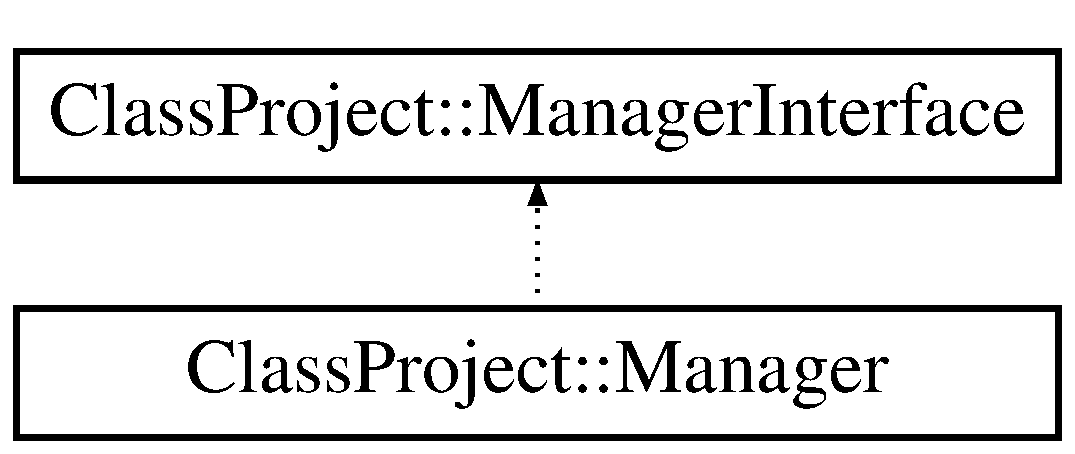
\includegraphics[height=2.000000cm]{classClassProject_1_1ManagerInterface}
\end{center}
\end{figure}
\subsection*{Public Member Functions}
\begin{DoxyCompactItemize}
\item 
virtual B\+D\+D\+\_\+\+ID {\bfseries create\+Var} (const std\+::string \&label)=0\label{classClassProject_1_1ManagerInterface_ab101acd3fbe6a5e29973d88f9862b8b4}

\item 
virtual const B\+D\+D\+\_\+\+ID \& {\bfseries True} ()=0\label{classClassProject_1_1ManagerInterface_a104d0e8bcbd81eb501b66db6e24d1f63}

\item 
virtual const B\+D\+D\+\_\+\+ID \& {\bfseries False} ()=0\label{classClassProject_1_1ManagerInterface_a98d18e1bc840fd664af015facfdcf690}

\item 
virtual bool {\bfseries is\+Constant} (const B\+D\+D\+\_\+\+ID f)=0\label{classClassProject_1_1ManagerInterface_a0edd879f6ecae7bc5f84a2d55373d977}

\item 
virtual bool {\bfseries is\+Variable} (const B\+D\+D\+\_\+\+ID x)=0\label{classClassProject_1_1ManagerInterface_a6eaaec7cbf8826198e490313ccb8f22a}

\item 
virtual B\+D\+D\+\_\+\+ID {\bfseries top\+Var} (const B\+D\+D\+\_\+\+ID f)=0\label{classClassProject_1_1ManagerInterface_ae2c645f859bcc7be3376d478f01eb045}

\item 
virtual B\+D\+D\+\_\+\+ID {\bfseries ite} (const B\+D\+D\+\_\+\+ID i, const B\+D\+D\+\_\+\+ID t, const B\+D\+D\+\_\+\+ID e)=0\label{classClassProject_1_1ManagerInterface_a6ea8f9482d86afb4128c52328d9ec11c}

\item 
virtual B\+D\+D\+\_\+\+ID {\bfseries co\+Factor\+True} (const B\+D\+D\+\_\+\+ID f, B\+D\+D\+\_\+\+ID x)=0\label{classClassProject_1_1ManagerInterface_aab8496a0e551abdad99160e152199f4b}

\item 
virtual B\+D\+D\+\_\+\+ID {\bfseries co\+Factor\+False} (const B\+D\+D\+\_\+\+ID f, B\+D\+D\+\_\+\+ID x)=0\label{classClassProject_1_1ManagerInterface_ad749ef1542c5b23bbbce628d6f666fe4}

\item 
virtual B\+D\+D\+\_\+\+ID {\bfseries co\+Factor\+True} (const B\+D\+D\+\_\+\+ID f)=0\label{classClassProject_1_1ManagerInterface_a4a1880d2245af9130646232551940949}

\item 
virtual B\+D\+D\+\_\+\+ID {\bfseries co\+Factor\+False} (const B\+D\+D\+\_\+\+ID f)=0\label{classClassProject_1_1ManagerInterface_a308c99661ad02f407d6f2b0af6230e80}

\item 
virtual B\+D\+D\+\_\+\+ID {\bfseries and2} (const B\+D\+D\+\_\+\+ID a, const B\+D\+D\+\_\+\+ID b)=0\label{classClassProject_1_1ManagerInterface_af914326d34a1ed42710f7b11e5baf010}

\item 
virtual B\+D\+D\+\_\+\+ID {\bfseries or2} (const B\+D\+D\+\_\+\+ID a, const B\+D\+D\+\_\+\+ID b)=0\label{classClassProject_1_1ManagerInterface_a8dbfde761b1e94d1f222b4d27f3c6fbc}

\item 
virtual B\+D\+D\+\_\+\+ID {\bfseries xor2} (const B\+D\+D\+\_\+\+ID a, const B\+D\+D\+\_\+\+ID b)=0\label{classClassProject_1_1ManagerInterface_a2b2c4948ef41ddb1036289cd07dac156}

\item 
virtual B\+D\+D\+\_\+\+ID {\bfseries neg} (const B\+D\+D\+\_\+\+ID a)=0\label{classClassProject_1_1ManagerInterface_a57d34af3121dcf5366d22ecf792f05a0}

\item 
virtual B\+D\+D\+\_\+\+ID {\bfseries nand2} (const B\+D\+D\+\_\+\+ID a, const B\+D\+D\+\_\+\+ID b)=0\label{classClassProject_1_1ManagerInterface_aaf6e357d680613e449d3ea958c9abba1}

\item 
virtual B\+D\+D\+\_\+\+ID {\bfseries nor2} (const B\+D\+D\+\_\+\+ID a, const B\+D\+D\+\_\+\+ID b)=0\label{classClassProject_1_1ManagerInterface_a312d9865eae2d6355e17855cba78bc78}

\item 
virtual std\+::string {\bfseries get\+Top\+Var\+Name} (const B\+D\+D\+\_\+\+ID \&root)=0\label{classClassProject_1_1ManagerInterface_afde45b2065361dfa6e61c1c7bc3fc1b4}

\item 
virtual void {\bfseries find\+Nodes} (const B\+D\+D\+\_\+\+ID \&root, std\+::set$<$ B\+D\+D\+\_\+\+ID $>$ \&nodes\+\_\+of\+\_\+root)=0\label{classClassProject_1_1ManagerInterface_ab460e331ffdb85d4128574b3aae72c1e}

\item 
virtual void {\bfseries find\+Vars} (const B\+D\+D\+\_\+\+ID \&root, std\+::set$<$ B\+D\+D\+\_\+\+ID $>$ \&vars\+\_\+of\+\_\+root)=0\label{classClassProject_1_1ManagerInterface_ab94feabca2125d334e542e502ae0186d}

\item 
virtual size\+\_\+t {\bfseries unique\+Table\+Size} ()=0\label{classClassProject_1_1ManagerInterface_a85cac80444b26e5b80eb96b9f1231c0e}

\end{DoxyCompactItemize}


The documentation for this class was generated from the following file\+:\begin{DoxyCompactItemize}
\item 
/import/home/vdscp04/\+Luiz/vdscp\+\_\+04/src/Manager\+Interface.\+h\end{DoxyCompactItemize}

%--- End generated contents ---

% Index
\backmatter
\newpage
\phantomsection
\clearemptydoublepage
\addcontentsline{toc}{chapter}{Index}
\printindex

\end{document}
